\documentclass[professionalfonts,table,serif,aspectratio=1610]{beamer}

\usepackage{newcent}
\usepackage[T1]{fontenc}
\usepackage[utf8]{inputenc}
\usepackage{amsmath,amssymb}
\usepackage{multicol,color}
\usepackage{beamerthemesplit}
\usepackage{graphicx,subfigure}
\usepackage{bm,bbm,bbding,units}
\hypersetup{colorlinks=true,allcolors=magenta}

\usepackage{texnames}
\usepackage{natbib}
\usepackage{tikz}
\usetikzlibrary{positioning}
\usetikzlibrary{arrows.meta}

\usetheme{Darmstadt}
\usecolortheme{seagull}
\setbeamercovered{transparent}
\setbeamertemplate{footline}[frame number]
\setbeamertemplate{navigation symbols}{}
\mode<handout>{
  \usepackage[bar]{beamerthemetree}
  \beamertemplatesolidbackgroundcolor{black!5}}

\renewcommand{\newblock}{}


\title{How to be Lucky Publishing}
\author[A.\ C.\ Frery ]{Alejandro C.\ Frery}
\institute[UFAL]{
\includegraphics[width=.3\linewidth]{laccan.pdf}\\
Instituto de Computação\\
Universidade Federal de Alagoas
}
\date{17 February 2017}

%\logo{\includegraphics[width=.04\linewidth]{ufal.eps}}

\setbeamercovered{dynamic}
%\AtBeginSection[]{\frame{\frametitle{Resumo}\tableofcontents[current]}}

\begin{document}

\begin{frame}{Acknowledgments}
This visit is only possible thanks to the kindness of \mbox{Prof.\ Xin Li} and colleagues, and the generosity of the Chinese Academy of Sciences.
\end{frame}

\begin{frame}{My trip}
\includegraphics[width=\linewidth]{MCZ-LHW-SYX-MIA-MCZ}
\end{frame}

\begin{frame}{Where do I come from? Maceió}
\includegraphics<1>[width=\linewidth]{./Figuras/PontaVerde}
\includegraphics<2>[width=\linewidth]{./Figuras/Piscinas1}
\includegraphics<3>[width=\linewidth]{./Figuras/Piscinas2}
\includegraphics<4>[width=\linewidth]{./Figuras/Barquinho}
\end{frame}

\frame{\titlepage}

\section{Introduction}

\begin{frame}
 \frametitle{Why publish?}
\begin{itemize}
\item<1-3> Vocation vs.\ Pressure
\item<1-3> Does it make sense?
\item<2-3> No, if it does not come with pleasure\dots\ that's why I chose \textcolor{red}{lucky} instead of \textcolor{red}{successful}.
\item<3> Lucky is successful \textcolor{red}{and} happy.
\end{itemize}
\end{frame}

\section{Before Submission}

\begin{frame}{What is a scientific article?}
A comprehensive summary of a research report published in a recognized venue.
\end{frame}

\begin{frame}{What is a scientific article?}
A comprehensive summary of a \textcolor{red}{research} report published in a recognized venue.
\end{frame}

\begin{frame}{What is research?}
\begin{itemize}[<+-| alert@+>]
\item Shaking the frontier of human knowledge
\item Where is such frontier?
	\begin{itemize}
	\item Complete, qualified and updated review of the literature
	\item JCR, top-class conferences, high quality books\dots
	\end{itemize}
\item Starts with a scientific question that
	\begin{itemize}
	\item has not been answered yet,
	\item can be answered with the time, materials and skills available,
	\item its progress can be measured and then reported.
	\end{itemize}
\end{itemize}
\end{frame}

\begin{frame}{What is a scientific article?}
A \textcolor{red}{comprehensive summary} of a research \textcolor{red}{report} published in a recognized venue.
\end{frame}

\begin{frame}{IMRaD}
A good structure for a scientific article is
\begin{itemize}
\item Introduction (delimitation, hypothesis)
\item Methodology (how I did what I did)
\item Results (what I observed doing what I did)
\item Discussion (how what I observed relates to the hypothesis)
\end{itemize}
\end{frame}

\begin{frame}{What is a scientific article?}
A comprehensive summary of a research report published in a \textcolor{red}{recognized venue}.
\end{frame}

\begin{frame}{What is a recognized venue?}
\begin{itemize}
\item JCR journals
\item Popularity and influence measures of performance
\end{itemize}
\end{frame}

\begin{frame}{How to choose and approach a journal}
\begin{itemize}[<+-| alert@+>]
\item It should be among the ones you read most
\item Know the Editorial Board (Editor-in-Chief, Associate Editors)
\item Do you analyze results already published in this journal?
\item Do you see your contribution published in this journal?
\item Prepare your submission following the guidelines
\end{itemize}
\end{frame}

\section{Preparation}

\begin{frame}{How to fail miserably a submission}
\begin{itemize}[<+-| alert@+>]
\item Bad English
\item Plagiarism
\item Multiple submission
\item Erring the public
\item Not specifying clearly the contribution
\item Making it as confusing as possible
\item Making it irreproducible
\item Making it ugly
\end{itemize}
\end{frame}

\begin{frame}{Recommendations}
\begin{alertblock}{Top tools}
\LaTeX, \BibTeX, \texttt R
\end{alertblock}

\begin{alertblock}{Strategy}
Reproducible Research, with SVN or Git
\end{alertblock}
\end{frame}

\begin{frame}
 \frametitle{Reproducible article}
It has to be associated to a Web page containing:
\begin{itemize}[<+-| alert@+>]
\item Title
\item Authors, with links to their Web pages
\item Summary
\item The PDF file, and information about its stage (in preparation, submitted, accepted, archived)
\item The data used and how to read them
\item All the code, including for data handling, and for producing figures and tables, well documented and with running examples.
\item Details on the computational platforms employed
\item E-mail and other ways of contact
\item List of references with their abstracts
\end{itemize}
\end{frame}

\begin{frame}
 \frametitle{Journals and RR}
The following journals \alert{at least} stimulate the use of RR:\\
IEEE Transactions on Image Processing, IEEE Transactions on Signal Processing, IEEE Transactions on Pattern Analysis and Machine Intelligence, IEEE Transactions on Neural Networks, International Journal of Computer Vision, Applied and Computational Harmonic Analysis, EURASIP Journal on Applied Signal Processing, BMC Bioinformatics, Journal of the Optical Society of America A, \href{http://www.jstatsoft.org/v34/i04}{Journal of Statistical Software}, Annals of Internal Medicine, The Insight Journal.

By the way, reviewers love to play with the code and data they are assessing.
These add great value to the submission. 
\end{frame}

\begin{frame}{Is \textbf{that} coming to the Remote Sensing community?}
\begin{alertblock}{Get ready I!}
In November 2016, the IEEE GRSS AdCom approved the creation of the ``\href{https://rscl-grss.org}{IEEE GRSS Remote Sensing Code Library},'' led by Inaugural Editor \mbox{Prof.\ F.\ T.\ Ulaby}, so\dots
\end{alertblock}

\begin{alertblock}{Get ready II!}
Authors have the option to upload their algorithms to \href{https://codeocean.com/ieee/signup}{Code Ocean}: a web service for uploading and sharing their algorithms and associated data, where other users are able to run them, and test modifications to the code.
Languages: \texttt{C/C++}, \texttt{Fortran}, \texttt{Java}, \texttt{Julia}, \texttt{Lua}, \texttt{Matlab}, \texttt{Octave}, \texttt{Perl}, \texttt{Python}, \texttt{R}.
\end{alertblock}
\end{frame}

\section{After Submission}

\begin{frame}{Flowchart}
\centering
\begin{tikzpicture}
[scale=.75,
caixa/.style={rectangle,draw,minimum height=10mm,minimum width=23mm,rounded corners},
circulo/.style={circle,draw,radius=12mm}]
%
\node (Accept) [circulo]{\textcolor{blue}{\textbf{Accept}}};
\node (Major) [caixa, below=of Accept] {Major Revision};
\node (Minor) [caixa, right=of Major] {Minor Revision};
\node (RejRes) [caixa, left=of Major] {Reject \& Resubmit};
\node (Reject) [circulo,below=of Major]{\textcolor{red}{\textbf{Reject}}};
%
\draw[->,thick,blue] (Major) -- (Accept);
\draw[->,thick,red] (Major) -- (Reject);
\draw[->,thick,red] (RejRes) -- (Reject);
\draw[->,thick,blue] (RejRes) -- (Accept);
\draw[->,thick,red] (Minor) -- (Reject);
\draw[->,thick,blue] (Minor) -- (Accept);
\draw[->,thick,blue] (Major.east) to [bend left=45] (Minor.west);
\draw[<-,thick,red] (Major.east) to [bend right=45] (Minor.west);
\draw[->,thick,blue] (RejRes.east) to [bend left=45] (Major.west);
\draw[<-,thick,red] (RejRes.east) to [bend right=45] (Major.west);
\draw[->,thick,blue,min distance=50mm] (RejRes.north) to [bend left=90] (Minor.north);
\draw[<-,thick,red,min distance=50mm] (RejRes.south) to [bend right=90] (Minor.south);
\end{tikzpicture}
\end{frame}

\begin{frame}
\frametitle{References}
\nocite{TenRulesReproducibleComputationalResearch,%
StatisticalAnalysesReproducibleResearch,%
EditorialGRSL2015,%
ManifestoReproducibleScience}
\bibliographystyle{agsm_url}
\bibliography{art04,art13,art17,rdt}
\end{frame}

{ % brace to limit the scope of \setbeamertemplate 
\setbeamertemplate{background canvas}{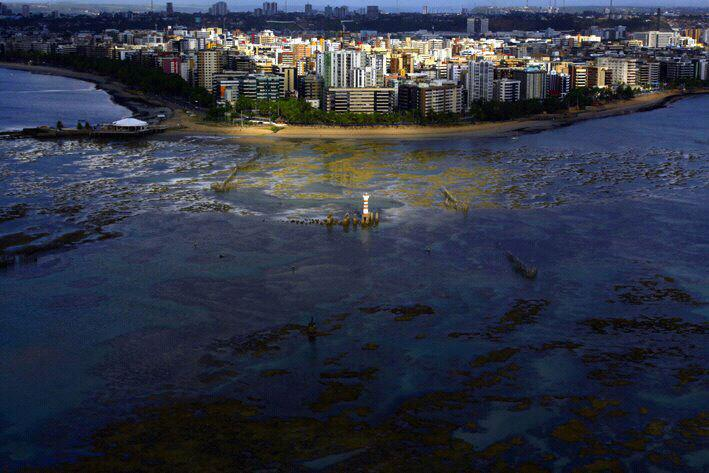
\includegraphics 
	[width=\paperwidth,height=\paperheight]{AmanhecerMaceio.jpg}} 

\begin{frame}[plain] 
\mbox{}\vskip12em
\begin{alertblock}{Contact:}
Alejandro C. Frery\\
\includegraphics[width=.5\linewidth]{AliChanChan}\\
\texttt{acfrery@gmail.com}\\
\texttt{http://sites.google.com/site/acfrery}\\
\HandRight~\framebox{MSc, PhD and Exchange Programs}~\HandLeft
\end{alertblock}
\end{frame} 
}

\end{document}